\documentclass{article}
\usepackage{graphicx} % Required for inserting images
\usepackage[top=0.9in, bottom=1in, left=1.5in, right=1.5in]{geometry}
\usepackage[utf8]{inputenc}
\usepackage[icelandic]{babel}
\usepackage[T1]{fontenc}
\usepackage[sc]{mathpazo}
\usepackage[parfill]{parskip}
% Tables and lists
\usepackage{booktabs,tabularx}
\usepackage{multirow}
\usepackage{enumerate}
\usepackage{adjustbox}
\usepackage{multicol}
\usepackage{xcolor}
\usepackage{algpseudocode}
\usepackage{hyperref}
\hypersetup{colorlinks=true}
\usepackage{tikz}
\usetikzlibrary{arrows, positioning, calc}

% Math
\usepackage{amsmath, amsfonts, amssymb, amsthm}
% Graphics

\usepackage{graphicx}
\usepackage{tikz}
% Code environment
\usepackage{minted}
%\usepackage{bm}
%\usepackage{siunitx}
%\usepackage{animate}
%\usepackage{hyperref}
%\usepackage{movie15}
%\usepackage{multicol}
%\usepackage{changepage}
\title{Tölvugrafík Heimadæmi 2}
\author{Ragnar Björn Ingvarsson, rbi3}

\begin{document}
	\maketitle
	\section{}
	\begin{itemize}
		\item[a.] \url{https://skogarbjorn.github.io/h2/1a/}

			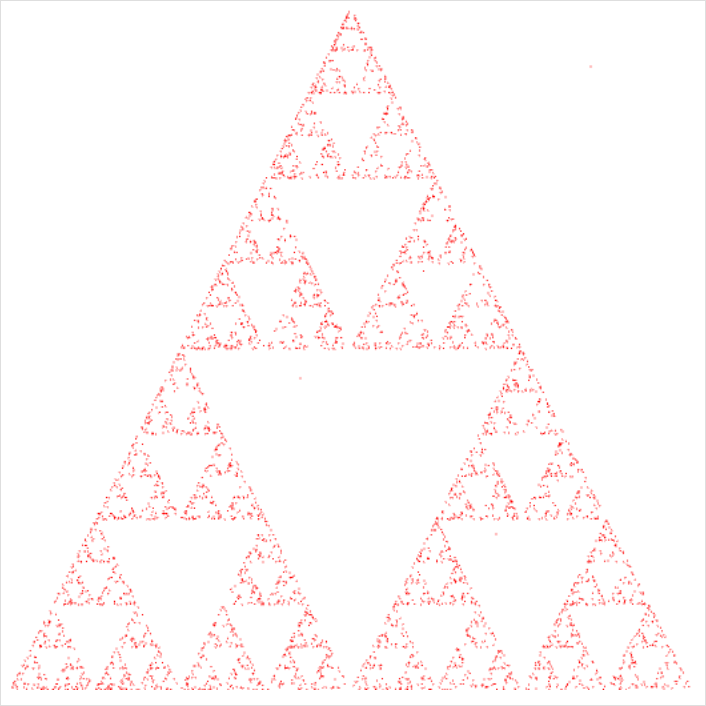
\includegraphics[scale=0.45]{far.png}

			\newpage
		\item[b.] \url{https://skogarbjorn.github.io/h2/1b/}

			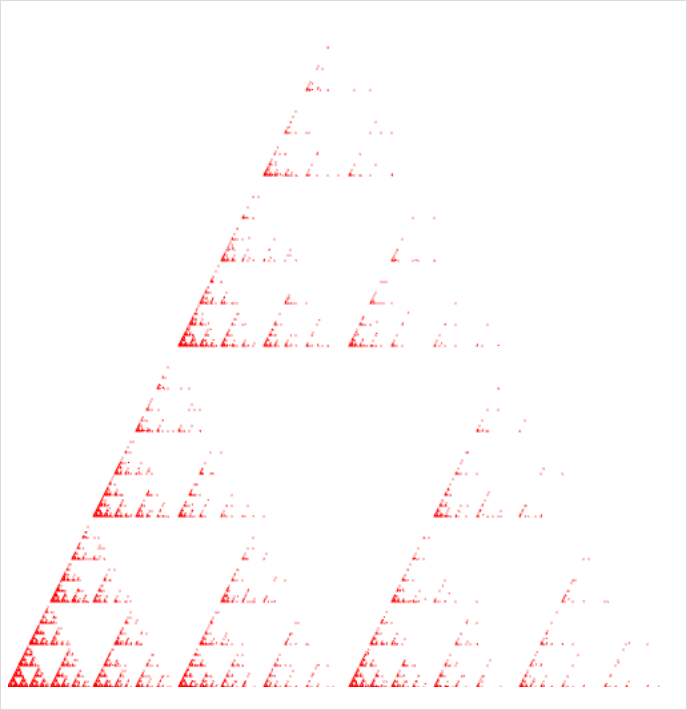
\includegraphics[scale=0.45]{weighted.png}

	\end{itemize}

	\section{}
	
	\url{https://skogarbjorn.github.io/h2/2a/circlefan.html}

	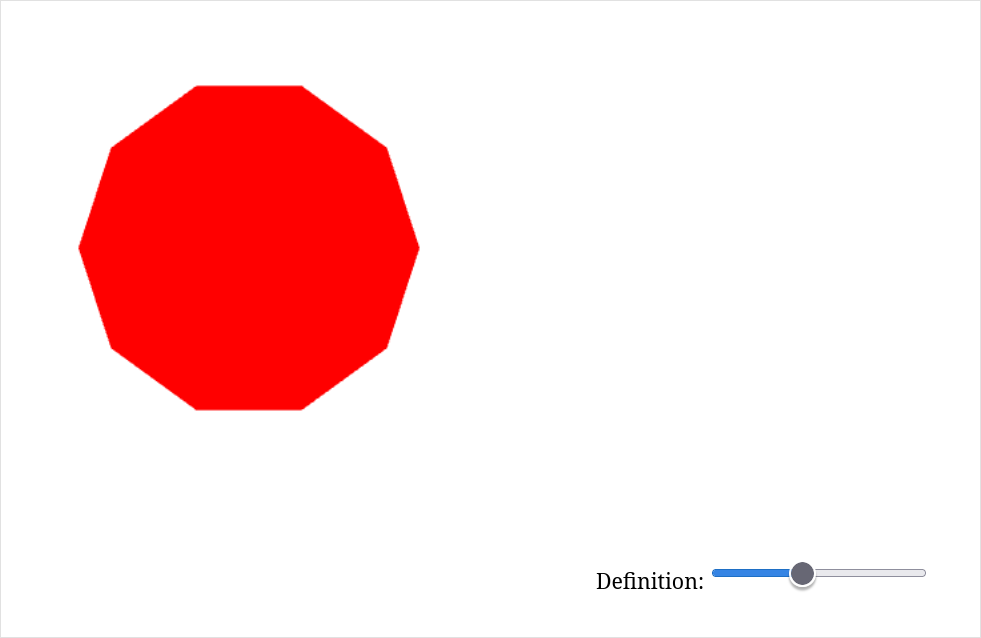
\includegraphics[scale=0.35]{circle.png}
			
	\section{}
	
	\url{https://skogarbjorn.github.io/h2/3a/L-shape-fan.html}
	
	\begin{center}
	
\includegraphics[scale=0.4]{l.png}
	\end{center}

	\section{}
	
	\url{https://skogarbjorn.github.io/h2/4a/clickcircles.html}

	\begin{center}
	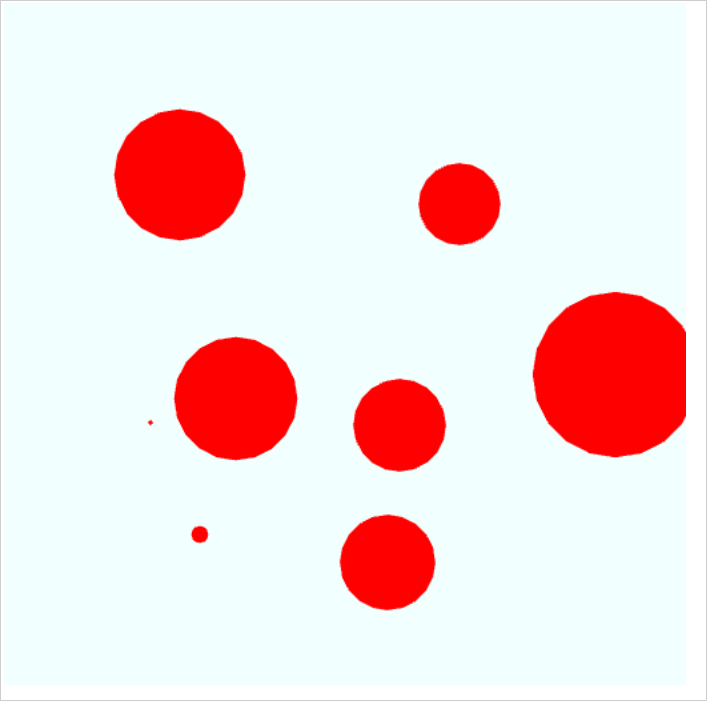
\includegraphics[scale=0.4]{circles.png}
	\end{center}

	\section{}
	
	\url{https://skogarbjorn.github.io/h2/5a/carpet.html}

	\begin{center}
	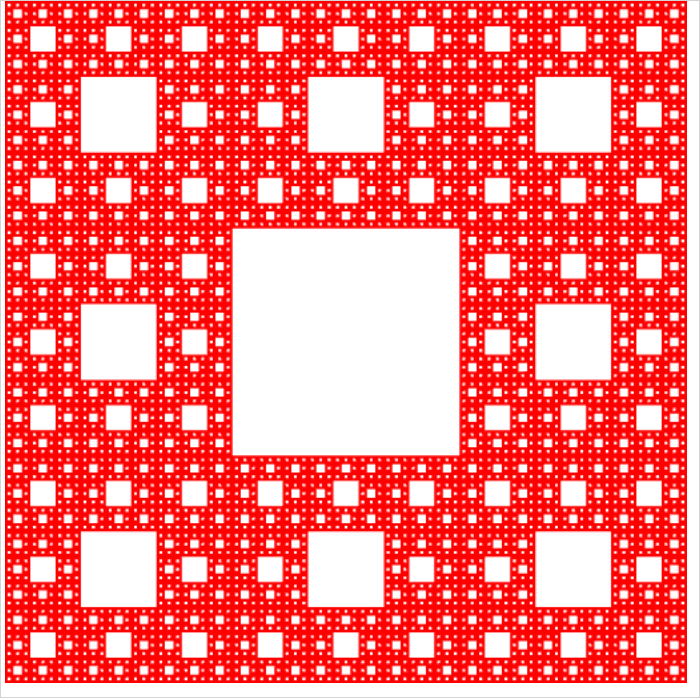
\includegraphics[scale=0.45]{carpet.png}
	\end{center}
\end{document}
